\documentclass{scrreprt}
\usepackage{listings}
\usepackage{underscore}
\usepackage{graphicx}
\usepackage[bookmarks=true]{hyperref}
\usepackage[utf8]{inputenc}
\usepackage[english]{babel}
\hypersetup{
    bookmarks=false,    % show bookmarks bar?
    pdftitle={Software Requirement Specification},    % title
    pdfauthor={Jean-Philippe Eisenbarth},                     % author
    pdfsubject={TeX and LaTeX},                        % subject of the document
    pdfkeywords={TeX, LaTeX, graphics, images}, % list of keywords
    colorlinks=true,       % false: boxed links; true: colored links
    linkcolor=blue,       % color of internal links
    citecolor=black,       % color of links to bibliography
    filecolor=black,        % color of file links
    urlcolor=purple,        % color of external links
    linktoc=page            % only page is linked
}%
\def\myversion{1.0 }
\date{}
%\title
\usepackage{hyperref}
\begin{document}

\begin{flushright}
    \rule{16cm}{5pt}\vskip1cm
    \begin{bfseries}
        \Huge{SOFTWARE REQUIREMENTS\\ SPECIFICATION IEEE 830}\\
        \vspace{1.5cm}
        for\\
        \vspace{1.5cm}
        Zenith PWA\\
        \LARGE{Version \myversion}\\
        \vspace{1.5cm}
        Prepared by : García Gonzalez Christian Andrés\\
        López Bautista Cristian Alexis\\
        Mercado Juárez Ángel Hayr\\
        Salas Díaz Guillermo\\
        Santillán Galavíz Ken Antonio\\
        \vspace{1.5cm}
        Submitted to : Dr. Ray Brunet Parra Galaviz \\
        \vspace{1.5cm}
        \today\\
    \end{bfseries}
\end{flushright}

\tableofcontents

\chapter{Introduction}

\section{Purpose}
The purpose of the "Zenith" project is to develop a Progressive Web Application (PWA) that extends the existing web platform's capabilities, specifically tailored for the use of businesses. The application aims to provide a comprehensive solution for managing and analyzing employee data, including personal and health information. The primary goal is to facilitate efficient incident reporting related to employees, covering both illnesses and workplace accidents. By leveraging the platform, organizations can maintain a centralized record of incidents and utilize graphical representations and tables for streamlined review and analysis.

\section{Intended Audience and Reading Suggestions}
The primary audience for the "Zenith" PWA includes businesses and organizations seeking an integrated solution for employee data management and incident reporting. This encompasses various stakeholders, such as human resources personnel, safety officers, and healthcare professionals within the organization. Additionally, those responsible for overseeing employee well-being and safety, such as nurses and health aides, will find the mobile capabilities of the application particularly beneficial.
\newline
\newline
Reading suggestions for this document are as follows:

\begin{itemize}
    \item Business executives and decision-makers: Focus on the overarching goals and benefits of the "Zenith" PWA in enhancing employee data management and incident reporting within the organization.
    \item Technical teams and developers: Explore the detailed specifications and requirements outlined in subsequent sections to understand the technical aspects of implementing the PWA.
    \item End users: Gain insights into the user experience and functionalities of the "Zenith" PWA, particularly if involved in incident reporting or data management.
\end{itemize}

\section{Project Scope}
The scope of the "Zenith" PWA project encompasses the development and deployment of a user-friendly and efficient platform for managing employee data and incident reporting.
\newline
\newline
Key features include:

\begin{itemize}
    \item Employee Data Management: Capture and store comprehensive employee information, including personal details, health data (e.g., blood type, allergies), and relevant contact information.
    \item Incident Reporting: Enable users to quickly and seamlessly report incidents through the mobile application, including details of illnesses and workplace accidents.
    \item Data Visualization: Provide graphical representations and tabular views of incident data for easy review and analysis by authorized personnel.
    \item Mobile Accessibility: Extend the platform's accessibility to mobile devices, allowing healthcare professionals and safety officers to scan unique employee QR codes for instant access to relevant information and incident reporting capabilities.
\end{itemize}

The "Zenith" PWA aims to enhance organizational efficiency, data accuracy, and emergency response by offering a comprehensive and accessible solution for managing employee information and incident reporting.

\chapter{Overall Description}

\section{Product Perspective}
The "Zenith" PWA is designed as an extension of the existing "Zenith" web platform, creating a seamless and integrated experience for users. The PWA interacts with the same backend infrastructure and database, ensuring consistency and real-time data synchronization between the web and mobile interfaces. The PWA is a self-contained system, but it relies on the web platform's data storage and processing capabilities.

\section{User Classes and Characteristics}
The "Zenith" PWA caters to different user classes with varying roles and responsibilities within an organization:

\begin{itemize}
    \item Administrators: Responsible for managing overall system settings, user access, and overseeing the integration with the existing web platform.
    \item Healthcare Professionals: Including nurses and health aides, these users focus on accessing and updating employee health information, as well as utilizing the incident reporting feature for quick response.
    \item Safety Officers: Tasked with monitoring and managing workplace safety, safety officers utilize the platform to review incident reports, analyze trends, and take preventive measures.
    \item Employees: Regular employees use the PWA to access their personal information, including health details, and report incidents quickly through the mobile interface.
\end{itemize}

\section{Product Functions}
The "Zenith" PWA incorporates the following key functions:

\begin{itemize}
    \item User Authentication and Authorization: Ensures secure access to the platform, with varying levels of permissions based on user roles.
    \item Employee Data Management: Allows administrators to add, modify, and delete employee information, including personal details and health-related data.
    \item Incident Reporting: Enables users to swiftly report incidents, providing details such as type of incident, location, and a brief description. Notifications are sent automatically to designated emergency contacts.
    \item Data Visualization: Presents graphical representations and tabular views of incident data, supporting trend analysis and decision-making.
    \item QR Code Scanning: Facilitates mobile accessibility by allowing healthcare professionals and safety officers to scan unique employee QR codes, providing instant access to relevant information and incident reporting features.
\end{itemize}

\section{Operating Environment}
The "Zenith" PWA operates in a web-based environment and is compatible with modern web browsers, ensuring accessibility across various devices and platforms. The application is designed to function efficiently in both online and offline modes, providing a seamless user experience even in low-connectivity scenarios.

\section{Design}
The design of the "Zenith" PWA focuses on an intuitive and user-friendly interface, ensuring a positive user experience. 

    \begin{figure}[h!]
      \centering
      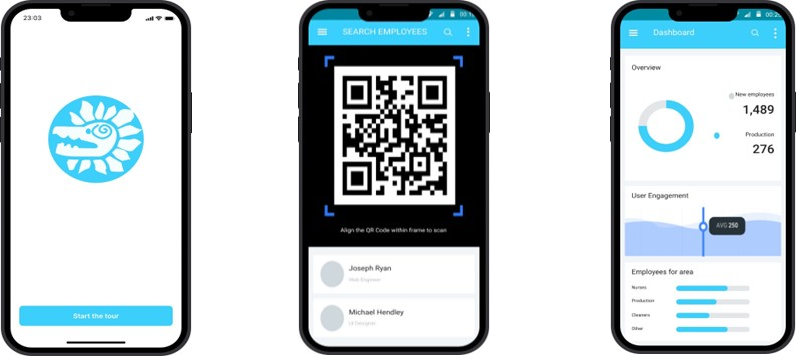
\includegraphics[width=0.75\textwidth]{mockups1.png}
      \caption{Zenith splash screem, QR scanning and charts.}
    \end{figure}

The mobile interface is optimized for responsiveness, allowing users to navigate and utilize features effortlessly on devices of varying screen sizes. Given the dynamic nature of security operations, personnel often need to access critical information on the go. The adaptability of our PWA to various mobile devices ensures that security consultations can be conducted seamlessly on smartphones and tablets, providing flexibility and efficiency in daily tasks.
\newline

    \begin{figure}[h!]
      \centering
      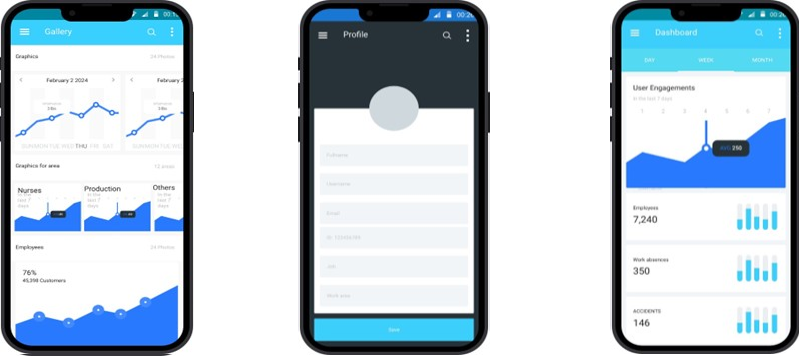
\includegraphics[width=0.75\textwidth]{mockups2.png}
      \caption{Zenith user data and profile page.}
    \end{figure}
    
The overall design adheres to industry best practices for security, scalability, and maintainability to support the long-term success of the platform.
\newline

    \begin{figure}[h!]
      \centering
      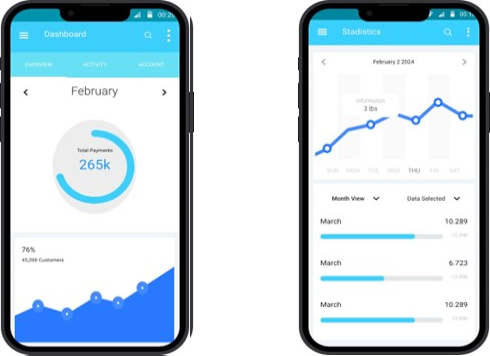
\includegraphics[width=0.75\textwidth]{mockups3.png}
      \caption{Zenith dashboards.}
    \end{figure}

\chapter{System Features}

\section{Description and Priority}
The "Zenith" PWA encompasses several key features crucial for efficient employee data management and incident reporting. Each feature is prioritized based on its significance to the overall functionality of the platform.

\begin{itemize}
    \item User Authentication and Authorization (Priority: High): Securely authenticate users and assign appropriate access levels based on their roles. Ensures data privacy and system integrity.
    \item Employee Data Management (Priority: High): Allows administrators to add, modify, and delete employee information, including personal details and health-related data. Ensures accurate and up-to-date records.
    \item Incident Reporting (Priority: High): Enables users to quickly report incidents, providing essential details such as incident type, location, and a brief description. Automatic notifications are sent to designated emergency contacts for swift response.
    \item Data Visualization (Priority: Medium): Presents incident data through graphical representations and tabular views, facilitating trend analysis and informed decision-making by safety officers and administrators.
    \item  Code Scanning (Priority: Medium): Facilitates mobile accessibility by allowing healthcare professionals and safety officers to scan unique employee QR codes. Provides instant access to employee information and incident reporting features.
\end{itemize}

\section{Functional Requirements}

\subsection{User Authentication and Authorization}

\begin{itemize}
    \item Requirement 1: Users must register with a valid email and password.
    \item Requirement 2: The system must verify user credentials securely before allowing access.
    \item Requirement 3: Different user roles (Administrator, Healthcare Professional, Safety Officer, Employee) must have distinct permissions.
\end{itemize}

\subsection{Employee Data Management}

\begin{itemize}
    \item Requirement 4: Administrators can add new employees, capturing personal details and health-related information.
    \item Requirement 5: Employee information must be editable to accommodate changes in personal or health data.
    \item Requirement 6: Administrators can delete employee records, ensuring data accuracy and compliance.
\end{itemize}

\subsection{Incident Reporting}

\begin{itemize}
    \item Requirement 7: Users can initiate incident reports, providing details such as incident type, location, and description.
    \item Requirement 8: The system must timestamp and store incident reports securely in the database.
    \item Requirement 9: Automated notifications must be sent to designated emergency contacts upon the submission of an incident report.
\end{itemize}

\subsection{Data Visualization}

\begin{itemize}
    \item Requirement 10: The system must generate graphical representations (charts, graphs) of incident data for easy visualization.
    \item Requirement 11: Tabular views of incident data must be available for detailed analysis.
    \item Requirement 12: Authorized users can apply filters for customized views based on parameters such as date, incident type, or employee.
\end{itemize}

\subsection{QR Code Scanning}

\begin{itemize}
    \item Requirement 13: The PWA must support QR code scanning functionality for quick access to employee information.
    \item Requirement 14: Scanned QR codes must provide healthcare professionals and safety officers with access to incident reporting features.
\end{itemize}

These functional requirements ensure the successful implementation of core features within the "Zenith" PWA, addressing the needs of various user classes and contributing to a comprehensive employee data management and incident reporting system.

\chapter{Other Nonfunctional Requirements}

\section{Performance Requirements}

\subsection{Response Time}

\begin{itemize}
    \item Requirement 1: The "Zenith" PWA should provide a responsive user interface, with an average response time of no more than 2 seconds for standard operations.
\end{itemize}

\subsection{Scalability}

\begin{itemize}
    \item Requirement 2: The system must handle a scalable number of users, supporting simultaneous access by at least 500 users without significant degradation in performance.
\end{itemize}

\section{Security Requirements}

\subsection{Data Encryption}

\begin{itemize}
    \item Requirement 3: All communication between the PWA and the backend system must be encrypted using secure protocols (e.g., HTTPS) to ensure data confidentiality.
\end{itemize}

\subsection{User Authentication}

\begin{itemize}
    \item Requirement 4: User authentication must comply with industry best practices, including secure password storage and protection against common authentication vulnerabilities.
\end{itemize}

\subsection{Authorization Controls}

\begin{itemize}
    \item Requirement 5: The system must enforce role-based access controls, ensuring that each user can only access features and data relevant to their assigned role.
\end{itemize}

\subsection{Incident Report Security}

\begin{itemize}
    \item Requirement 6: Incident reports must be stored securely, and access to this sensitive information must be restricted to authorized personnel.
\end{itemize}

\section{Software Quality Attributes}

\subsection{Usability}

\begin{itemize}
    \item Requirement 7: The PWA must be designed with a user-friendly interface, ensuring ease of navigation and a positive user experience for individuals with varying levels of technical proficiency.
\end{itemize}

\subsection{Reliability}

\begin{itemize}
    \item Requirement 8: The system must have a high level of reliability, with an expected uptime of at least 99\% to minimize disruptions to user access.
\end{itemize}

\subsection{Maintainability}

\begin{itemize}
    \item Requirement 9: The codebase must be well-documented, and the system architecture should allow for easy maintenance and updates without significant downtime.
\end{itemize}

\section{Business Rules}

\subsection{Incident Reporting}

\begin{itemize}
    \item Requirement 10: Employees are required to report any work-related incidents within 24 hours of occurrence.
    \item Requirement 11: Incident reports must include accurate and detailed information to be considered valid.
\end{itemize}

\subsection{Data Accuracy}

\begin{itemize}
    \item Requirement 12: Employee data must be reviewed and updated by administrators annually to ensure accuracy.
    \item Requirement 13: Inaccurate or outdated data must be corrected promptly upon identification.
\end{itemize}


\chapter{Other Requirements}

\section{Cross-Browser Compatibility}

\begin{itemize}
    \item Requirement 1: The PWA should be compatible with popular web browsers, including but not limited to Google Chrome, Mozilla Firefox, Safari, and Microsoft Edge, to ensure a consistent user experience.
\end{itemize}

\section{Mobile Device Compatibility}

\begin{itemize}
    \item Requirement 2: The PWA must be optimized for mobile devices, supporting various screen sizes and resolutions to facilitate ease of use on smartphones and tablets.
\end{itemize}

\section{Training and Documentation}

\begin{itemize}
    \item Requirement 3: Comprehensive training materials and documentation must be provided to assist users in understanding the functionalities of the PWA, promoting efficient system usage.
\end{itemize}


\end{document}